\documentclass[10pt,a4paper,onecolumn]{article}
% \usepackage[utf8]{inputenc}
\usepackage{marginnote}
\usepackage{graphicx}
\usepackage{xcolor}
\usepackage{authblk,etoolbox}
\usepackage{titlesec}
\usepackage{calc}
\usepackage{hyperref}
\hypersetup{breaklinks=true,
            bookmarks=true,
            pdfauthor=
{
      Guillaume Viejo,
      Benoît Girard,
      Mehdi Khamassi,
  },
            pdftitle=
{
[Re] Speed/accuracy trade-off between the habitual and the goal-directed
processes
},
            colorlinks=true,
            citecolor=blue,
            urlcolor=blue,
            linkcolor=blue,
            pdfborder={0 0 0}}
\urlstyle{same}
\usepackage{tcolorbox}
\usepackage{ragged2e}
\usepackage{fontspec}
\usepackage{fontawesome}
\usepackage{caption}
\usepackage{listings}
\lstnewenvironment{code}{\lstset{language=Haskell,basicstyle=\small\ttfamily}}{}



%\usepackage{fancyvrb}
%\VerbatimFootnotes
%\usepackage{graphicx}
%\usepackage{mdframed}
%\newmdenv[backgroundcolor=lightgray]{Shaded}


\usepackage{longtable,booktabs}

\usepackage[
  backend=biber,
%  style=alphabetic,
%  citestyle=numeric
]{biblatex}
\bibliography{viejo_girard_khamassi.bib}



% --- Macros ------------------------------------------------------------------
\renewcommand*{\bibfont}{\small \sffamily}

\definecolor{red}{HTML}{CF232B}
\newcommand{\ReScience}{Re{\bfseries \textcolor{red}{Science}}}

\newtcolorbox{rebox}
   {colback=blue!5!white, colframe=blue!40!white,
     boxrule=0.5pt, arc=2pt, fonttitle=\sffamily\scshape\bfseries,
     left=6pt, right=20pt, top=6pt, bottom=6pt}

\newtcolorbox{repobox}
   {colback=red, colframe=red!75!black,
     boxrule=0.5pt, arc=2pt, left=6pt, right=6pt, top=3pt, bottom=3pt}

% fix for pandoc 1.14     
\newcommand{\tightlist}{%
  \setlength{\itemsep}{1pt}\setlength{\parskip}{0pt}\setlength{\parsep}{0pt}}

% --- Style -------------------------------------------------------------------
\renewcommand*{\bibfont}{\small \sffamily}
\renewcommand{\captionfont}{\small\sffamily}
\renewcommand{\captionlabelfont}{\bfseries}

\makeatletter
\renewcommand\@biblabel[1]{{\bf #1.}}
\makeatother

% --- Page layout -------------------------------------------------------------
\usepackage[top=3.5cm, bottom=3cm, right=1.5cm, left=1.5cm,
            headheight=2.2cm, reversemp, includemp, marginparwidth=4.5cm]{geometry}

% --- Section/SubSection/SubSubSection ----------------------------------------
\titleformat{\section}
  {\normalfont\sffamily\Large\bfseries}
  {}{0pt}{}
\titleformat{\subsection}
  {\normalfont\sffamily\large\bfseries}
  {}{0pt}{}
\titleformat{\subsubsection}
  {\normalfont\sffamily\bfseries}
  {}{0pt}{}
\titleformat*{\paragraph}
  {\sffamily\normalsize}


% --- Header / Footer ---------------------------------------------------------
\usepackage{fancyhdr}
\pagestyle{fancy}
%\renewcommand{\headrulewidth}{0.50pt}
\renewcommand{\headrulewidth}{0pt}
\fancyhead[L]{\hspace{-1cm}\includegraphics[width=4.0cm]{rescience-logo.pdf}}
\fancyhead[C]{}
\fancyhead[R]{} 
\renewcommand{\footrulewidth}{0.25pt}

\fancyfoot[L]{\hypersetup{urlcolor=red}
              \sffamily \ReScience~$\vert$
              \href{http://rescience.github.io}{rescience.github.io}
              \hypersetup{urlcolor=blue}}
\fancyfoot[C]{\sffamily \thepage}
\fancyfoot[R]{\sffamily Sep 2015 $\vert$
                        Volume \textbf{1} $\vert$
                        Issue \textbf{1}}
\pagestyle{fancy}
\makeatletter
\let\ps@plain\ps@fancy
\fancyheadoffset[L]{4.5cm}
\fancyfootoffset[L]{4.5cm}

% --- Title / Authors ---------------------------------------------------------
% patch \maketitle so that it doesn't center
\patchcmd{\@maketitle}{center}{flushleft}{}{}
\patchcmd{\@maketitle}{center}{flushleft}{}{}
% patch \maketitle so that the font size for the title is normal
\patchcmd{\@maketitle}{\LARGE}{\LARGE\sffamily}{}{}
% patch the patch by authblk so that the author block is flush left
\def\maketitle{{%
  \renewenvironment{tabular}[2][]
    {\begin{flushleft}}
    {\end{flushleft}}
  \AB@maketitle}}
\makeatletter
\renewcommand\AB@affilsepx{ \protect\Affilfont}
%\renewcommand\AB@affilnote[1]{{\bfseries #1}\hspace{2pt}}
\renewcommand\AB@affilnote[1]{{\bfseries #1}\hspace{3pt}}
\makeatother
\renewcommand\Authfont{\sffamily\bfseries}
\renewcommand\Affilfont{\sffamily\small\mdseries}
\setlength{\affilsep}{1em}

\LetLtxMacro{\OldIncludegraphics}{\includegraphics}
\renewcommand{\includegraphics}[2][]{\OldIncludegraphics[width=12cm, #1]{#2}}


% --- Document ----------------------------------------------------------------
\title{[Re] Speed/accuracy trade-off between the habitual and the goal-directed
processes}

    \usepackage{authblk}
                        \author[1]{Guillaume Viejo}
                    \author[1]{Benoît Girard}
                    \author[1]{Mehdi Khamassi}
                            \affil[1]{Sorbonne Universités, UPMC Univ Paris 06, CNRS, Institute of Intelligent
Systems and Robotics (ISIR), F-75005 Paris, France}
            
\date{\vspace{-5mm}
      \sffamily \small \href{mailto:guillaume.viejo@isir.upmc.fr}{guillaume.viejo@isir.upmc.fr}}


\setlength\LTleft{0pt}
\setlength\LTright{0pt}


\begin{document}
\maketitle

\marginpar{
  %\hrule
  \sffamily\small
  %\vspace{2mm}
  {\bfseries Editor}\\
  Name Surname\\

  {\bfseries Reviewers}\\
        Name Surname\\
        Name Surname\\
  
  {\bfseries Received}  Nov, 1, 2015\\
  {\bfseries Accepted}  Sep, 1, 2015\\
  {\bfseries Published} Sep, 1, 2015\\

  {\bfseries Licence}   \href{http://creativecommons.org/licenses/by/4.0/}{CC-BY}

  \begin{flushleft}
  {\bfseries Competing Interests:}\\
  The authors have declared that no competing interests exist.
  \end{flushleft}

  \hrule
  \vspace{3mm}

  \hypersetup{urlcolor=white}
  
    \vspace{-1mm}
  \begin{repobox}
    \bfseries\normalsize
      \href{http://github.com/rescience/rescience-submission/article}{\faGithubAlt~Article repository}
  \end{repobox}
      \vspace{-1mm}
  \begin{repobox}
    \bfseries\normalsize
      \href{http://github.com/rescience/rescience-submission/code}{\faGithubAlt~Code repository}
  \end{repobox}
        \hypersetup{urlcolor=blue}
}

\begin{rebox}
\sffamily {\bfseries A reference implementation of}
\small
\begin{flushleft}
\begin{itemize}
    \item[→] Speed/accuracy trade-off between the habitual and the goal-directed
processes, M. Keramati, A. Dezfouli, P. Payam, PLoS computational
biology, 7, 2011
  \end{itemize}\par
\end{flushleft}
\end{rebox}


\section{Introduction}\label{introduction}

This study is a reference implementation of \textcite{keramati} that
proposed an arbitration mechanism between a goal-directed strategy and a
habitual strategy, used to model the behavior of rats in instrumental
conditionning tasks. The habitual strategy is the Kalman Q-Learning from
\textcite{geist}. We replicate the results of the first task i.e.~the
devaluation experiment with two states and two actions. The
implementation is in python with numpy, scipy and matplotlib library.
The authors couldn't provide the original implementation and we are not
aware of others implementations elsewhere.

\section{Methods}\label{methods}

We used the description of the model from the original article except
for the implementation of the Kalman Q-Learning which we took from
\textcite{geist}. We used the same parameters as the original article
except for the update rate of the transition function \(\phi\), the
initialization of the covariance matrice and an uncentered transform
parameter \(\kappa\) that were not mentionned in the original article.
The largest uncertainty about the model concerned the devaluation
procedure. Besides setting the reward \(r\) to null, the authors stated
that ``For modeling the devaluation of the outcome in the first two
simulations, \(R(S_1, EM)\) is set to -1.'' As this notation
(\(R(S_1, EM)\)) is not defined in the rest of the article, we assumed
that it is \(\hat{R}(S_1, EM)\) updated by equation (14) in the original
article.

The parameters are as follows :

\begin{longtable}[c]{@{}lll@{}}
\toprule
Name & Description & Value\tabularnewline
\midrule
\endhead
\(\sigma\) & Updating rate of the average reward & 0.02\tabularnewline
\(\eta\) & Variance of evolution noise & 0.0001\tabularnewline
\(P_n\) & Variance of observation noise & 0.05\tabularnewline
\(\beta\) & Rate of exploration & 1.0\tabularnewline
\(\rho\) & Update rate of the reward function & 0.1\tabularnewline
\(\gamma\) & Discount factor & 0.95\tabularnewline
\(\tau\) & Time step of graph exploration & 0.08\tabularnewline
depth & Depth of search in graph exploration & 3\tabularnewline
\(\phi\) & Update rate of the transition function & 0.5\tabularnewline
init cov & Initialisation of covariance matrice & 1.0\tabularnewline
\(\kappa\) & Unscentered transform parameters & 0.1\tabularnewline
\bottomrule
\end{longtable}

We describe the algorithm of our implementation in details. The process
of action selection and reward update are separated for clarity.

\begin{quote}
\textbf{Initialization}
\end{quote}

\begin{quote}
\begin{quote}
\(Q(s, a)^{Goal-Directed} = \{ 0, \ldots \}\)
\end{quote}
\end{quote}

\begin{quote}
\begin{quote}
\(Q(s, a)^{Habitual} = \{ 0, \dots \}\)
\end{quote}
\end{quote}

\begin{quote}
\begin{quote}
\(\#\) Covariance matrix
\end{quote}
\end{quote}

\begin{quote}
\begin{quote}
\(\Sigma = \left(  \begin{array}{*4{c}}  cov \times \eta & 0 & \ldots & 0 \\  0 & cov \times \eta & \ldots & \vdots \\  \vdots & \ldots & \ddots & 0 \\  0 & \ldots & 0 & cov \times \eta \\  \end{array}\right)\)
\end{quote}
\end{quote}

\begin{quote}
\begin{quote}
\(R(S1, EM) = 1\) \(\#\) Reward value
\end{quote}
\end{quote}

\begin{quote}
\begin{quote}
\(\bar{R} = 0\) \(\#\) Reward rate
\end{quote}
\end{quote}

\begin{quote}
\begin{quote}
\(\hat{R}(s,a) = \{0,\ldots\}\) \(\#\) Reward function
\end{quote}
\end{quote}

\begin{quote}
\textbf{Main Loop}
\end{quote}

\begin{quote}
\begin{quote}
\(\textbf{FOR}\ i = 1:T\)
\end{quote}
\end{quote}

\begin{quote}
\begin{quote}
\begin{quote}
\(s_t = S_0\) \(\#\) Initial state
\end{quote}
\end{quote}
\end{quote}

\begin{quote}
\begin{quote}
\begin{quote}
\(\textbf{IF}\ i = T_{devaluation}\) \(\#\) Moderate / Extensive
training
\end{quote}
\end{quote}
\end{quote}

\begin{quote}
\begin{quote}
\begin{quote}
\begin{quote}
\(R(S1, EM) = 0\)
\end{quote}
\end{quote}
\end{quote}
\end{quote}

\begin{quote}
\begin{quote}
\begin{quote}
\begin{quote}
\(\hat{R}(S1, EM) = -1\)
\end{quote}
\end{quote}
\end{quote}
\end{quote}

\begin{quote}
\begin{quote}
\begin{quote}
\(\textbf{WHILE}\ s_t \neq S1 \bigwedge a_t \neq EM\)
\end{quote}
\end{quote}
\end{quote}

\begin{quote}
\begin{quote}
\begin{quote}
\begin{quote}
\(a_t = \textbf{Selection}(s_t)\)
\end{quote}
\end{quote}
\end{quote}
\end{quote}

\begin{quote}
\begin{quote}
\begin{quote}
\begin{quote}
\(r_t = R(s_t,a_t)\)
\end{quote}
\end{quote}
\end{quote}
\end{quote}

\begin{quote}
\begin{quote}
\begin{quote}
\begin{quote}
\(s_{t+1} = transition(s_t, a_t)\)
\end{quote}
\end{quote}
\end{quote}
\end{quote}

\begin{quote}
\begin{quote}
\begin{quote}
\begin{quote}
\(\textbf{Update}(s_t,a_t, s_{t+1}, r_t)\)
\end{quote}
\end{quote}
\end{quote}
\end{quote}

\begin{quote}
\textbf{Selection}
\end{quote}

\begin{quote}
\begin{quote}
\(\#\) Sort the Q-values in descending order
\end{quote}
\end{quote}

\begin{quote}
\begin{quote}
\(\{a_1,\ldots,ai,\ldots\} \leftarrow sort(Q(s_t,a_i))\)
\end{quote}
\end{quote}

\begin{quote}
\begin{quote}
\(\#\) VPI : Value of Precise Information
\end{quote}
\end{quote}

\begin{quote}
\begin{quote}
\(VPI(s_t, a_1) = (Q(s_t,a_2)^{H}-Q(s_t,a_1)^{H})P(Q(s_t,a_1)^{H}<Q(s_t,a_2)^{H})+ \frac{\sigma(s_t,a_t)}{\sqrt{2\pi}} e^{-\frac{(Q(s_t,a_2)^H - Q(s_t,a_1)^H)^2}{2\sigma(s_t,a_t)^2}}\)
\end{quote}
\end{quote}

\begin{quote}
\begin{quote}
\(VPI(s_t, a_i) = (Q(s_t,a_i)^{H}-Q(s_t,a_1)^{H})P(Q(s_t,a_i)^{H}>Q(s_t,a_1)^{H}) + \frac{\sigma(s_t,a_t)}{\sqrt{2\pi}} e^{-\frac{(Q(s_t,a_1)^H - Q(s_t,a_i)^H)^2}{2\sigma(s_t,a_t)^2}}\)
\end{quote}
\end{quote}

\begin{quote}
\begin{quote}
\(\textbf{FOR}\ i \in \{a_1, a_2,\ldots, a_i, \ldots\}\)
\end{quote}
\end{quote}

\begin{quote}
\begin{quote}
\begin{quote}
\(\textbf{IF}\ VPI(s_t, a_i) \geq \tau \bar{R}\)
\end{quote}
\end{quote}
\end{quote}

\begin{quote}
\begin{quote}
\begin{quote}
\begin{quote}
\(\#\) Q-Value from Goal-directed system is evaluated
\end{quote}
\end{quote}
\end{quote}
\end{quote}

\begin{quote}
\begin{quote}
\begin{quote}
\begin{quote}
\(Q(s_t,a_i) = \hat{R}(s_t,a_i) + \gamma \sum\limits_{s'}p_{T}(\{s,a\}\rightarrow s') \max\limits_{b \in A} Q(s',b)^{Goal-directed}\)
\end{quote}
\end{quote}
\end{quote}
\end{quote}

\begin{quote}
\begin{quote}
\begin{quote}
\(\textbf{ELSE}\)
\end{quote}
\end{quote}
\end{quote}

\begin{quote}
\begin{quote}
\begin{quote}
\begin{quote}
\(\#\) Q-Value from Habitual system is retrieved
\end{quote}
\end{quote}
\end{quote}
\end{quote}

\begin{quote}
\begin{quote}
\begin{quote}
\begin{quote}
\(Q(s_t,a_i) = Q(s_t,a_i)^{Habitual}\)
\end{quote}
\end{quote}
\end{quote}
\end{quote}

\begin{quote}
\begin{quote}
\(a_t \leftarrow \textit{SoftMax}(Q(s_t,a), \beta)\)
\end{quote}
\end{quote}

\begin{quote}
\textbf{Update}
\end{quote}

\begin{quote}
\begin{quote}
\(\bar{R} = (1-\sigma) \bar{R} + \sigma r_t\) \(\#\) Reward Rate
\end{quote}
\end{quote}

\begin{quote}
\begin{quote}
\(\hat{R}(s_t,a_t) =(1 - \rho) \hat{R} + \rho r_t\) \(\#\) Reward
function
\end{quote}
\end{quote}

\begin{quote}
\begin{quote}
\(p_{T}(s_t, a_t, s_{t+1}) = (1 - \phi) p_{T}(s_t, a_t, s_{t+1}) + \phi\)
\(\#\) Probability of transition
\end{quote}
\end{quote}

\begin{quote}
\begin{quote}
Specific to Kalman Q-Learning
\end{quote}
\end{quote}

\begin{quote}
\begin{quote}
\(\#\) Sigma-points sampling
\end{quote}
\end{quote}

\begin{quote}
\begin{quote}
\(\Theta = \{ \theta_j, 0 \geq j \geq 2|S.A|\}\)
\end{quote}
\end{quote}

\begin{quote}
\begin{quote}
\(\check{W} = \{ w_j, 0 \geq j \geq 2|S.A| \}\)
\end{quote}
\end{quote}

\begin{quote}
\begin{quote}
\(\check{R} = \{ \check{r}_j = \theta_j(s_t,a_t) - \gamma \max\limits_{b \in A} \theta_j(s_{t+1},b),\ 0 \geq j \geq 2|S.A|\}\)
\end{quote}
\end{quote}

\begin{quote}
\begin{quote}
\(r_{predicted} = \sum\limits_{j=0}^{2|S.A|} w_j \check{r}_j\)
\end{quote}
\end{quote}

\begin{quote}
\begin{quote}
\(\#\) Covariance computation
\end{quote}
\end{quote}

\begin{quote}
\begin{quote}
\(P_{\theta_j \check{r}_j} = \sum\limits_{j=0}^{2|S.A|} w_j (\theta_j - Q^{Habitual}_t)(\check{r}_j - r_{predicted})\)
\end{quote}
\end{quote}

\begin{quote}
\begin{quote}
\(P_{\check{r}_j} = \sum\limits_{j=0}^{2|S.A|} w_j (\check{r}_j - r_{predicted})^2 + P_n\)
\end{quote}
\end{quote}

\begin{quote}
\begin{quote}
\(K_t = P_{\theta_j \check{r}_j} P_{\check{r}_j}^{-1}\) \(\#\) Kalman
gain
\end{quote}
\end{quote}

\begin{quote}
\begin{quote}
\(\delta_t = r_t - r_{predicted}\) \(\#\) Reward-prediction error
\end{quote}
\end{quote}

\begin{quote}
\begin{quote}
\(Q_{t+1}^{Habitual} = Q_{t}^{H} + K_t \delta_t\)
\end{quote}
\end{quote}

\begin{quote}
\begin{quote}
\(P_{t+1}^{H} = P_{t}^{H} - K_t P_{\Sigma_t} K_t^T\)
\end{quote}
\end{quote}

\section{Results}\label{results}

We only reproduced the results of Figure 3 A, B, G, H in a qualitative
manner. Results are presented in Figure \ref{fig:figure1}. We can
observe the strategy shift (from goal-directed to habitual) after
extensive training around 50 time steps. In the original article, the
strategy shift occurs after 100 time steps.

However we can observe a difference between the probabilities of action
for the goal-directed model. In our implementation,
\[p(s_0, pl) \simeq 0.7\] and \[p(s_0, em) \simeq 0.3\] before
devaluation. In the original article, \[p(s_0, pl) \simeq 0.6\] and
\[p(s_0, em) \simeq 0.4\] Nevertheless, the probabilities of action from
the Kalman Q-Learning after strategy shifting are equivalent.

\begin{figure}[htbp]
\centering
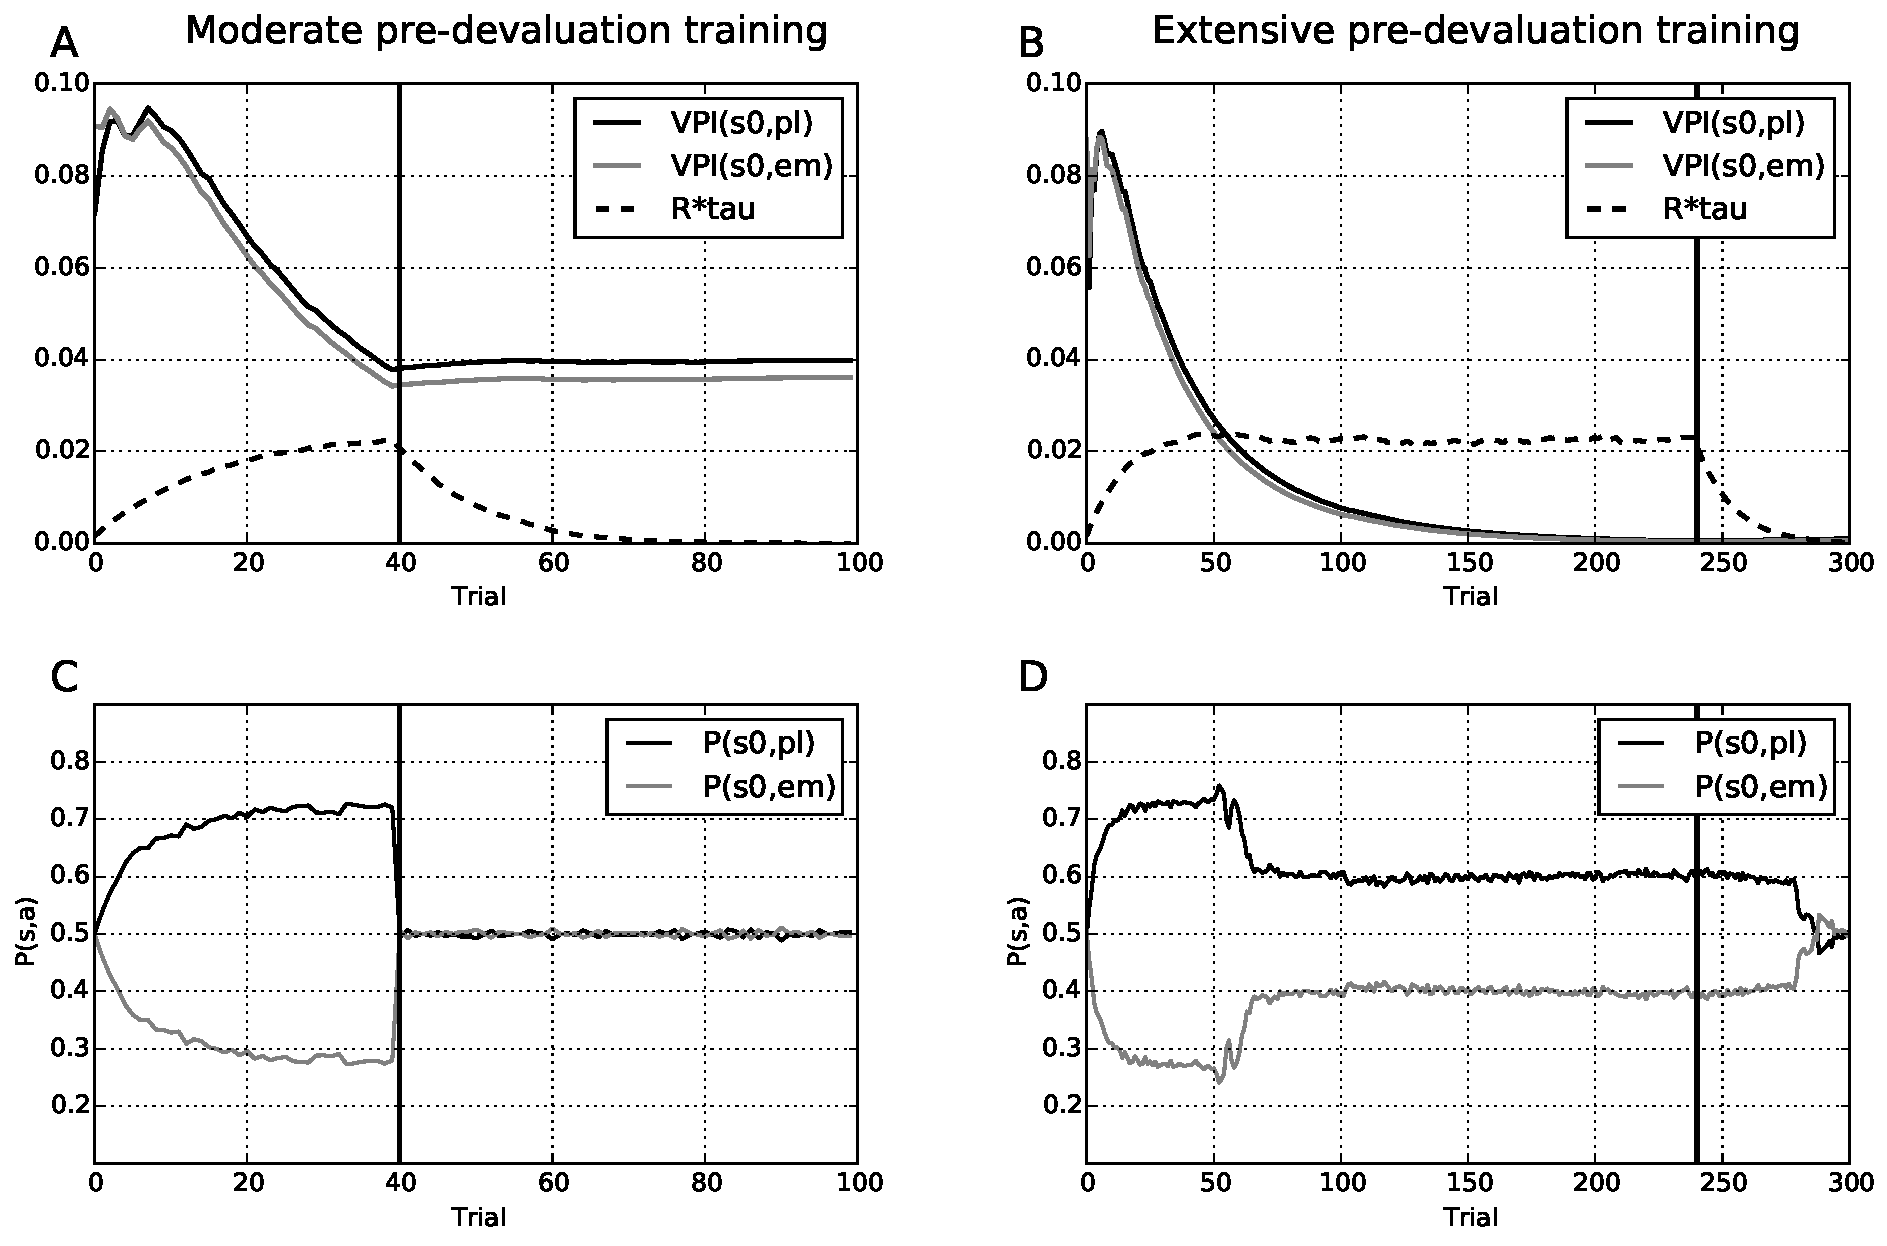
\includegraphics{../code/fig.pdf}
\caption{\label{fig:figure1}A. Value of Precise Information (full lines)
for action press-lever and enter magazine in state \(S_0\) and reward
rate (dashed line) in moderate training. Vertical line represents the
timing of devaluation. B. In extensive training. C. Probability of
actions in state \(S_0\) in moderate training. D. In extensive
training.}
\end{figure}

\section{Conclusion}\label{conclusion}

We were able to qualitatively reproduce the first simulations of the
article. Despite the small differences in the exact timing of the
strategy shifting and in the probabilities of action, the behavior of
our implementation is similar to the original article. Thus, we confirm
the correctness of the model presented in the original article.

{\sffamily \small
  \printbibliography[title=References]
}
\end{document}
